\chapter{CÔNG TRÌNH NGHIÊN CỨU LIÊN QUAN}
\label{chap:lienquan}
Chương này đối chiếu các phương án tích hợp CPU và bộ tăng tốc CNN để làm rõ lựa chọn kiến trúc MyTinyMobileNetSoC. Trọng tâm là phân công công việc, đường truyền dữ liệu và nơi tái sử dụng toán hạng, thay vì liệt kê đặc tính của từng lõi hoặc từng khối phần cứng. Phạm vi hệ thống của luận văn được xác định ở Chương~\ref{chap:gioithieu}; kiến trúc và kết quả tối ưu tương ứng được trình bày ở Chương~\ref{chap:kientruc} và Chương~\ref{chap:toiuu}.

\section{Tiêu chí so sánh và các phương án kiến trúc}
\label{sec:related-criteria}
Một bộ tăng tốc có nhiều đơn vị nhân--cộng chưa đủ bảo đảm suy luận nhanh nếu việc chuẩn bị và chuyển toán hạng chiếm nhiều thời gian. Vì vậy, chương sử dụng các tiêu chí sau để đặt các công trình trên cùng một khung phân tích:
\begin{enumerate}
    \item \textbf{Phân công CPU/phần cứng:} CPU chỉ khởi phát một tác vụ lớn hay còn dựng cửa sổ, cấp toán hạng, cộng bias và hoàn thiện từng đầu ra?
    \item \textbf{Điều khiển và truyền dữ liệu:} lệnh tùy chỉnh, thanh ghi MMIO, DMA, cache hay runtime đảm nhiệm phần nào; bộ tăng tốc có tự truy cập bộ nhớ hay không?
    \item \textbf{Phạm vi toán tử và số học:} tích chập chuẩn, depthwise, pointwise, FC, pooling và lượng tử hóa được hỗ trợ tới đâu; độ rộng tensor và tích lũy có tương đồng không?
    \item \textbf{Tái sử dụng và bộ nhớ:} trọng số, cửa sổ đầu vào và tổng riêng được giữ ở đâu; lịch tính toán cần bộ đệm, băng thông và dung lượng lưu trữ nào?
    \item \textbf{Bằng chứng đánh giá:} workload, đối chứng và ranh giới đo là gì; kết quả đến từ mô phỏng, hiện thực vật lý hay đo trên bo mạch?
\end{enumerate}

Theo các tiêu chí này, có thể đối chiếu ba hướng: ngoại vi tính toán do CPU cấp dữ liệu; bộ đồng xử lý nhận lệnh và chủ động chuyển dữ liệu qua hệ thống nhớ; và các kernel FPGA do trình biên dịch/runtime điều phối. Ge và cộng sự cung cấp trường hợp SoC với bộ đệm chuyên dụng~\cite[Sections~3--4]{ge2019compact}; He minh họa tích hợp RoCC cùng DMA~\cite[Section~3]{he2021design}; Chung khảo sát tổ chức kernel và lịch thực thi OpenCL~\cite[Chapters~3--5]{chung2021optimization}. Các hướng này là những lựa chọn về mức tự chủ và chi phí tích hợp, không tạo thành thứ hạng hiệu năng chung.

Các bảng cuối chương chỉ tổng hợp đặc điểm có thể đối chiếu. Số liệu khác workload, độ chính xác số học hoặc công nghệ hiện thực không được dùng để suy ra ưu thế của MyTinyMobileNetSoC. Đặc biệt, thông lượng nhân ma trận cực đại không đồng nghĩa độ trễ của cả mạng, còn số chu kỳ mô phỏng không thay thế phép đo thời gian và năng lượng trên bo mạch.

\section{Lõi RISC-V gọn nhẹ và tích hợp bộ tăng tốc}
\subsection{PicoRV32 và giao tiếp bus gốc}
PicoRV32 là lõi RISC-V hướng tới diện tích nhỏ, có các lựa chọn giao tiếp bộ nhớ gốc, AXI4-Lite và Wishbone. Lõi thực hiện lệnh qua nhiều chu kỳ, không phải lõi đơn chu kỳ; thời gian còn phụ thuộc cấu hình và đáp ứng của bộ nhớ. Giao tiếp gốc dùng cơ chế valid/ready, phù hợp để kết nối RAM và ngoại vi qua bộ giải mã địa chỉ~\cite[README: Variants; PicoRV32 Native Memory Interface; Cycles per Instruction]{YosysHQ2024}.

Trong MyTinyMobileNetSoC, lựa chọn có ý nghĩa là giữ CPU làm chủ giao dịch và đưa các phép tính ra ngoại vi MMIO. Firmware dùng lệnh tải/lưu thông thường để nạp thanh ghi, khởi phát tính toán và đọc kết quả; không sử dụng giao diện lệnh đồng xử lý PCPI cho các toán tử CNN. Kiến trúc này cho phép quan sát rõ chi phí phục vụ dữ liệu, nhưng mỗi toán hạng phải đi qua CPU. RAM dùng chung chứa mã và tensor không đồng nghĩa ngoại vi được quyền tự đọc RAM, như sẽ mô tả ở Chương~\ref{chap:kientruc}.

Tài liệu PicoRV32 công bố tài nguyên và tần số cho những cấu hình lõi cụ thể~\cite[README: Features; Performance]{YosysHQ2024}. Những kết quả đó không đại diện cho SoC có RAM, bộ giải mã và các datapath CNN. Do đó, luận văn đánh giá tài nguyên và timing của toàn bộ thiết kế sau định tuyến ở Chương~\ref{chap:toiuu}, thay vì áp thông số lõi độc lập cho hệ thống tích hợp.

\subsection{Rocket/RoCC như một phương án đối chiếu}
Trong hệ sinh thái Rocket Chip, RoCC cho phép bộ tăng tốc nhận lệnh tùy chỉnh cùng toán hạng thanh ghi và trả kết quả về CPU. Bộ tăng tốc có thể dùng giao diện tới cache L1 hoặc kết nối TileLink tới hệ thống nhớ; lựa chọn đường truy cập ảnh hưởng thông lượng và độ phức tạp tích hợp~\cite{chipyardRoCC}. Cần phân biệt đường \emph{điều khiển} qua lệnh RoCC với đường \emph{dữ liệu} qua cache hoặc cổng nhớ: có RoCC không tự động có nghĩa mọi thiết kế đều dùng cùng một cơ chế DMA.

Khác với phương án đó, MyTinyMobileNetSoC không mở rộng tập lệnh để điều khiển CNN và không có DMA ở các ngoại vi. Cách tiếp cận này đổi lại sự đơn giản của giao diện phần mềm bằng chi phí tải/lưu và điều phối trên PicoRV32. Ngược lại, khả năng chuyển khối dữ liệu của bộ đồng xử lý đòi hỏi thêm điều khiển bộ nhớ và bộ đệm. Vì vậy, lựa chọn CPU trong chương được xem xét cùng phương thức tích hợp; danh mục pipeline hay hiệu năng lõi riêng không đủ để lựa chọn kiến trúc tăng tốc.

\section{Khảo sát về hiện thực bộ tăng tốc mạng CNN trên phần cứng}
\subsection{Compact Convolutional Neural Network Accelerator for IoT Endpoint SoC}
\subsubsection{Khối tích chập}
\begin{figure}[!h]
    \centering
    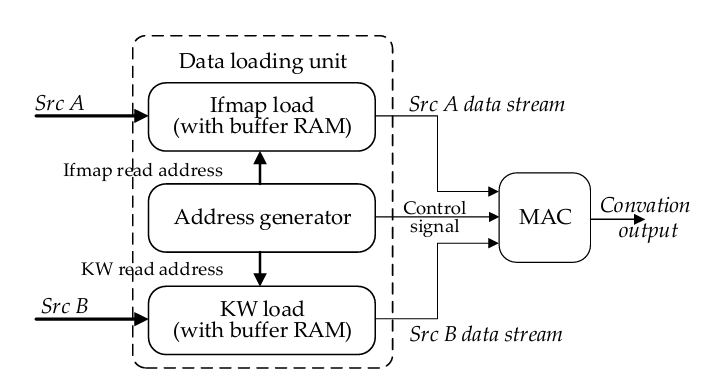
\includegraphics[width=0.5\textwidth]{Images/CNNAccelerator/CompactCNNAccelerator/conv_architecture.png}
    \vspace{10pt} % Thay đổi giá trị 10pt theo nhu cầu
    \caption{Kiến trúc của khối tích chập}
\end{figure}
Flow hoạt động của khối tích chập được thể hiện ở hình bên dưới:
\begin{figure}[!h]
    \centering
    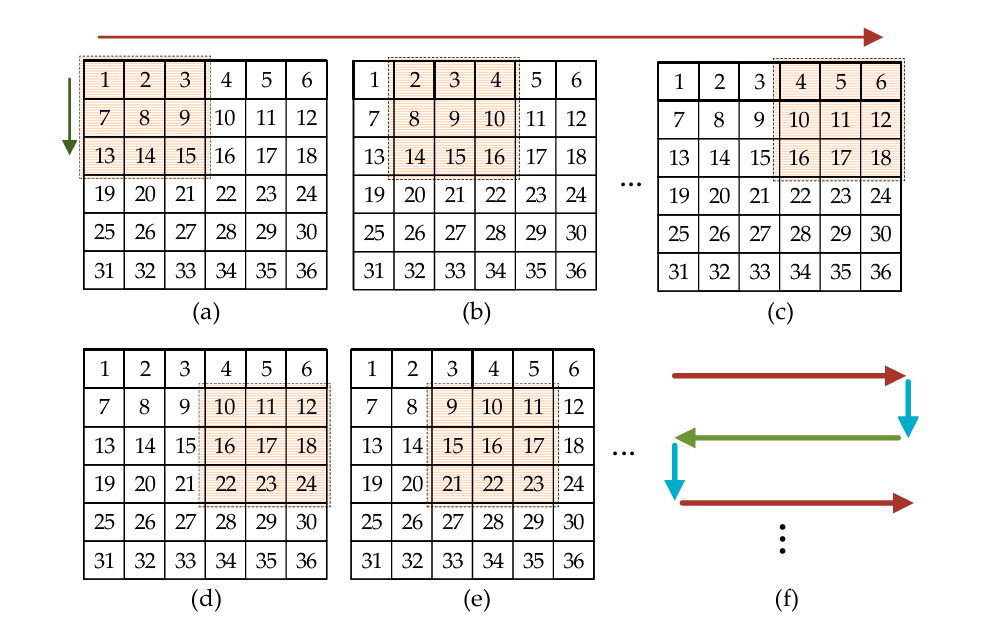
\includegraphics[width=0.7\textwidth]{Images/CNNAccelerator/CompactCNNAccelerator/conv_workflow.png}
    \vspace{10pt} % Thay đổi giá trị 10pt theo nhu cầu
    \caption{Workflow của khối tích chập}
\end{figure}

\begin{itemize}
    \item Đây là thành phần quan trọng nhất trong bộ gia tốc CNN vì CNN chủ yếu sử dụng phép toán tích chập. Thiết kế của đơn vị tích chập tập trung vào tối ưu hóa việc tải và lưu trữ dữ liệu.
    \item Sử dụng kỹ thuật giảm băng thông bộ nhớ bằng cách tận dụng sự lặp lại của dữ liệu trong phép toán tích chập, giúp giảm bớt băng thông cần thiết và tăng tốc độ tính toán.
    \item Các tín hiệu đầu vào được xử lý qua một bộ nhớ đệm (buffer RAM) để tối ưu hóa việc truy xuất dữ liệu.
\end{itemize}
\subsubsection{Khối Pooling}
Kiến trúc tổng quát của khối max-pooling được thể hiện ở sơ đồ bên dưới: 
\begin{figure}[!h]
    \centering
    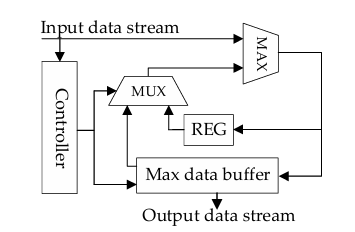
\includegraphics[width=0.5\textwidth]{Images/CNNAccelerator/CompactCNNAccelerator/pooling_architecture.png}
    \vspace{10pt} % Thay đổi giá trị 10pt theo nhu cầu
    \caption{Kiến trúc của khối pooling}
\end{figure}
\begin{itemize}
    \item Khối max-pooling thực hiện phương pháp max-pooling, giúp giảm kích thước dữ liệu đầu ra sau khi qua phép toán tích chập.
    \item Thiết kế của khối max-pooling là một mạch nối tiếp với bộ chọn và bộ so sánh (max comparator), cho phép giảm thiểu tài nguyên nhưng vẫn đảm bảo hiệu năng tính toán.
\end{itemize}
\subsubsection{Khối Multifunctional Accumulation Unit}
 Khối này được sử dụng để tích lũy kết quả của nhiều phép tích chập 2D. Nó cũng được chia sẻ với lớp bias, đơn giản hóa thiết kế và giảm tiêu thụ tài nguyên.
\subsubsection{Thiết kế chuỗi tăng tốc}
Chuỗi tăng tốc được thể hiện ở sơ đồ bên dưới:
\begin{figure}[!h]
    \centering
    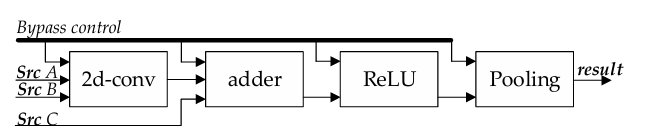
\includegraphics[width=0.5\textwidth]{Images/CNNAccelerator/CompactCNNAccelerator/chain_architecture.png}
    \vspace{10pt} % Thay đổi giá trị 10pt theo nhu cầu
    \caption{Kiến trúc của chuỗi tăng tốc}
\end{figure}
Bộ tăng tốc CNN được thiết kế theo dạng chuỗi gia tốc để tối ưu hóa hiệu suất tính toán. Mỗi chuỗi tăng tốc có thể thực hiện nhiều phép toán cùng lúc, giảm bớt sự di chuyển của dữ liệu giữa các phép toán và tăng hiệu suất tính toán. Cấu trúc của chuỗi tăng tốc bao gồm:
\begin{itemize}
    \item 4 chuỗi tăng tốc (acceleration chains): Mỗi chuỗi có thể thực hiện một phép toán tích chập độc lập, đồng thời giảm thiểu sự trùng lặp trong việc sử dụng tài nguyên.
    \item Kênh dữ liệu (Data Channels): Mỗi chuỗi gia tốc sử dụng các kênh dữ liệu như Src A, Src B, Src C, và kênh kết quả để chia sẻ thông tin giữa các thành phần khác nhau của bộ gia tốc.
\end{itemize}
Thiết kế này giúp xử lý song song nhiều lớp CNN với hiệu suất cao, đồng thời tiết kiệm tài nguyên bộ nhớ và giảm tiêu thụ năng lượng.\\
Bộ tăng tốc sử dụng một hệ thống điều khiển bypass để bỏ qua các module không cần thiết trong mỗi lớp mạng CNN, nhằm tối ưu hóa tốc độ xử lý. Các phép toán cũng được điều chỉnh độ rộng dữ liệu để phù hợp với kiến trúc 10-bit fixed-point, điều này giúp tiết kiệm tài nguyên mà không ảnh hưởng lớn đến độ chính xác. Bảng bên dưới cho thấy ảnh hưởng của độ rộng dữ liệu đối với độ chính xác của thuật toán là không đáng kể.
\subsubsection{Kiến trúc bộ tăng tốc}
Kiến trúc tổng quát của bộ tăng tốc được thể hiện ở sơ đồ bên dưới:
\begin{figure}[!h]
    \centering
    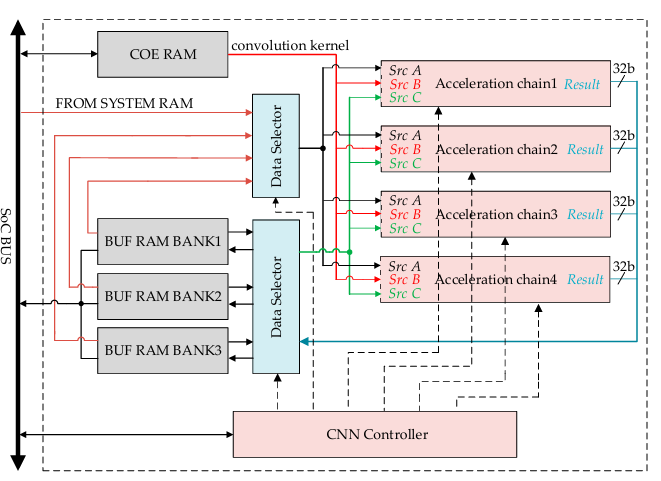
\includegraphics[width=0.7\textwidth]{Images/CNNAccelerator/CompactCNNAccelerator/accelerator_architecture.png}
    \vspace{10pt} % Thay đổi giá trị 10pt theo nhu cầu
    \caption{Kiến trúc của bộ tăng tốc}
\end{figure}
\begin{itemize}
    \item Bộ tăng tốc bao gồm bộ điều khiển CNN, ba khối đệm, bốn chuỗi tăng tốc và bộ chọn dữ liệu.
    \item Kiến trúc cho phép bộ tăng tốc thực hiện đồng thời các phép tích chập, kích hoạt và lấy mẫu con với bốn nhân tích chập dựa trên việc sử dụng ma trận nguồn, tăng hiệu suất tính toán.
    \item Bộ nhớ BUF RAM BANK được sử dụng để lưu trữ psum, ma trận nguồn và kết quả đệm, giảm thiểu việc di chuyển dữ liệu và tăng hiệu suất hệ thống. Mỗi BUF RAM BANK được ghép nối từ bốn SP-RAM độc lập để tăng băng thông truy cập.
    \item Bảng bên dưới tóm tắt các thông số cơ bản của bộ tăng tốc, cho thấy nó có thể đáp ứng các yêu cầu nhận dạng hình ảnh chung của SoC đầu cuối IoT.
\end{itemize}
\subsubsection{Thực nghiệm}
Để kiểm tra tính khả thi và hiệu quả của bộ gia tốc thiết kế, nhóm tác giả đã thực hiện một loạt thử nghiệm trên nền tảng FPGA, mô phỏng một hệ thống SoC (System-on-Chip) với bộ xử lý Cortex-M3.\\
Nền tảng thử nghiệm sử dụng vi xử lý ARM Cortex-M3 và chạy mạng Lenet-5 làm ví dụ.. Các thành phần chính của nền tảng thử nghiệm bao gồm:
\begin{itemize}
    \item Nền tảng được xây dựng dựa trên lõi Cortex-M3, một lõi MCU phổ biến của ARM cung cấp sự cân bằng tốt giữa hiệu suất và mức tiêu thụ năng lượng.
    \item SoC thử nghiệm bao gồm 128 KB RAM, 128 KB ROM và các thiết bị ngoại vi thông thường như GPIO và UART.
    \item SoC sử dụng bus AHB và APB để kết nối các thiết bị với lõi, với các thiết bị tốc độ cao như SCCB và bộ tăng tốc CNN được kết nối thông qua bus AHB, trong khi các thiết bị tốc độ thấp như GPIO được kết nối thông qua bus APB.
    \item Bảng dưới cho thấy mức tiêu thụ tài nguyên LUT của SoC khi được tổng hợp và triển khai trên FPGA. Bộ tăng tốc CNN chiếm 4901 LUT, chiếm tỷ lệ đáng kể trong tổng mức tiêu thụ tài nguyên của SoC.
\end{itemize}
Triển khai mạng kiểm thử Lenet-5
\begin{itemize}
    \item Mạng Lenet-5 được sử dụng để đánh giá bộ tăng tốc CNN. Lenet-5 là một mạng CNN cổ điển với các lớp tích chập (convolution layers), lớp gộp (subsampling), và lớp kết nối đầy đủ (fully connected). Việc triển khai mạng Lenet-5 trên nền tảng thử nghiệm giúp kiểm tra khả năng của bộ gia tốc trong việc xử lý các tác vụ nhận diện hình ảnh.
\end{itemize}
Kết quả thực nghiệm:
\begin{itemize}
    \item Hiệu suất của bộ tăng tốc được so sánh với CPU Intel i5 7500 và hai bộ xử lý ứng dụng di động Samsung S5P6818 và AllWinner H3
    \item Thời gian thực thi của Lenet-5 được đo trên các nền tảng khác nhau và được hiển thị ở bên dưới:
    \begin{figure}[!h]
    \centering
    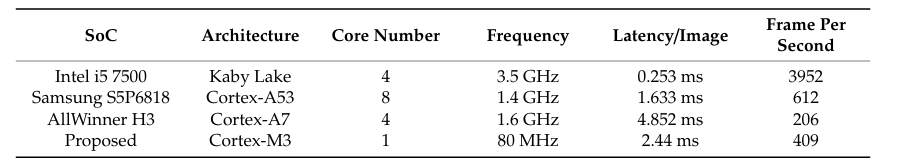
\includegraphics[width=\textwidth]{Images/CNNAccelerator/CompactCNNAccelerator/performance_table.png}
    \vspace{10pt} % Thay đổi giá trị 10pt theo nhu cầu
    \caption{Hiệu năng}
\end{figure}
\end{itemize}
Mức tiêu thụ tài nguyên:
Bài báo so sánh mức tiêu thụ tài nguyên của bộ tăng tốc được đề xuất với các bộ tăng tốc khác được báo cáo trong các tài liệu tham khảo:
\begin{itemize}
    \item Zhang, Y.; Wu, N.; Zhou, F.; Yahya, M.R. Design of Multifunctional Convolutional Neural Network Accelerator for IoT Endpoint SoC. In Proceedings of the World Congress on Engineering and Computer Science 2018, San Francisco, CA, USA, 23–25 October 2018; pp. 16–19.
    \item  Li, Z.; Wang, L.; Guo, S.; Deng, Y.; Dou, Q.; Zhou, H.; Lu, W. Laius: An 8-bit fixed-point CNN hardware inference engine. In Proceedings of the 2017 IEEE International Symposium on Parallel and Distributed Processing with Applications and 2017 IEEE International Conference on Ubiquitous Computing and Communications (ISPA/IUCC), Guangzhou, China, 12–15 December 2017; pp. 143–150.
    \item  Guo,K.; Sui, L.; Qiu, J.; Yu, J.; Wang, J.; Yao, S.; Han, S.; Wang, Y.; Yang, H. Angel-Eye: A complete design flow for mapping CNN onto embedded FPGA. IEEETrans. Comput. Des. Integr. Circuits Syst. 2018, 37, 35–47.
\end{itemize}
Kết quả được hiển thị ở bảng bên dưới:
\begin{figure}[!h]
    \centering
    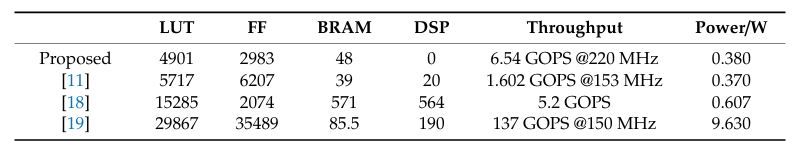
\includegraphics[width=0.7\textwidth]{Images/CNNAccelerator/CompactCNNAccelerator/resource_consumption_table.png}
    \vspace{10pt} % Thay đổi giá trị 10pt theo nhu cầu
    \caption{Mức tiêu thụ tài nguyên}
\end{figure}





\subsection{Optimization of Compiler-Generated OpenCL CNN Kernels and runtime for FPGAs}
\subsubsection{Triển khai mạng đầu cuối}
Sơ đồ luồng biên dịch được thể hiện ở hình bên dưới:
\begin{figure}[!h]
    \centering
    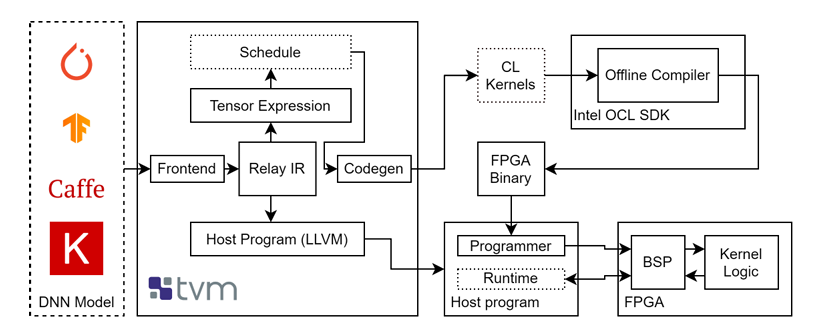
\includegraphics[width=\textwidth]{Images/CNNAccelerator/OptimizingCompiler-GeneratedOpenCLforCNNs/compilation_flow.png}
    \vspace{10pt} % Thay đổi giá trị 10pt theo nhu cầu
    \caption{Sơ đồ luồng biên dịch}
\end{figure}
\begin{itemize}
    \item Đầu vào: Mô hình CNN từ các framework ML khác nhau.
    \item TVM - một công cụ biên dịch tối ưu hóa cho học sâu, chuyển đổi mô hình thành biểu diễn trung gian (Relay IR).
    \item Biên dịch: TVM tạo mã OpenCL C từ Relay IR, sử dụng các hàm tính toán và lịch biểu được tối ưu hóa từ TVM Operator Inventory (TOPI).
    \item Tổng hợp: Intel OpenCL SDK tổng hợp mã OpenCL C thành phần cứng FPGA.
    \item Thực thi: Luồng dữ liệu được tạo trên FPGA để thực thi mô hình CNN.
\end{itemize}
Luồng biên dịch hỗ trợ hai chế độ thực thi: thực thi theo đường ống (pipelined) và thực thi gấp (folded).
\begin{itemize}
    \item Thực thi theo đường ống: Các bản đồ đặc trưng đầu ra được chuyển giữa các kernel bằng cách sử dụng các kênh OpenCL.
    \item Thực thi gấp: Các kernel được tham số hóa (hình dạng tensor đầu vào/đầu ra động) được sử dụng lại cho nhiều lớp trong mạng, tiêu thụ ít tài nguyên FPGA hơn so với thiết kế đường ống đầy đủ.
\end{itemize}
\subsubsection{Tối ưu hóa kernel OpenCL}
Các vấn đề với kernel OpenCL được tạo bởi trình biên dịch TVM:
\begin{itemize}
    \item Sử dụng bộ nhớ toàn cục không hiệu quả: Dẫn đến hiệu suất thấp do băng thông bộ nhớ toàn cục hạn chế.
    \item Sử dụng logic không hiệu quả: Dẫn đến việc sử dụng tài nguyên cao, làm cho các thiết kế lớn hơn không thể tổng hợp được.
    \item Tính song song thấp: Dẫn đến hiệu suất kém.
\end{itemize}
Các biện pháp tối ưu hóa được đề xuất:
\begin{itemize}
    \item Đọc coalesced: Kết hợp nhiều lần đọc nhỏ thành các lần đọc rộng hơn, cải thiện việc sử dụng băng thông bộ nhớ toàn cục.
    \item Lặp unrolling: Nhân rộng thân vòng lặp để tăng tính song song.
    \item Lặp fusion: Kết hợp nhiều vòng lặp thành một vòng lặp để giảm chi phí điều khiển vòng lặp và cải thiện cục bộ bộ nhớ cache.
    \item Di chuyển mã bất biến: Di chuyển các tính toán bất biến ra khỏi vòng lặp để giảm chi phí tính toán.
    \item Ghi bộ nhớ cache: Ghi kết quả trung gian vào bộ nhớ cục bộ để giảm truy cập bộ nhớ toàn cục.
    \item Kênh: Sử dụng kênh OpenCL để truyền dữ liệu giữa các kernel, giảm chi phí truyền dữ liệu bộ nhớ toàn cục và tăng tính song song.
    \item Kernel Autorun: Cho phép các kernel không có trọng số hoặc độ lệch thực thi ngay khi bộ đệm đầy, tăng tính song song.
    \item Thực thi đồng thời: Sử dụng nhiều hàng đợi lệnh để cho phép các kernel chạy song song, tăng hiệu suất.
    \item Kernel được tham số hóa: Nhóm và tham số hóa các kernel tương tự để chúng có thể được sử dụng lại trên toàn mạng, giảm mức sử dụng tài nguyên.
    \item Tối ưu hóa hoạt động dấu phẩy động: Sử dụng các tối ưu hóa do Intel OpenCL SDK cung cấp để cải thiện hiệu suất của các hoạt động dấu phẩy động.
\end{itemize}
Các phương pháp tối ưu hóa và khả năng áp dụng của chúng được thể hiện ở hình bên dưới.
\begin{figure}[!h]
    \centering
    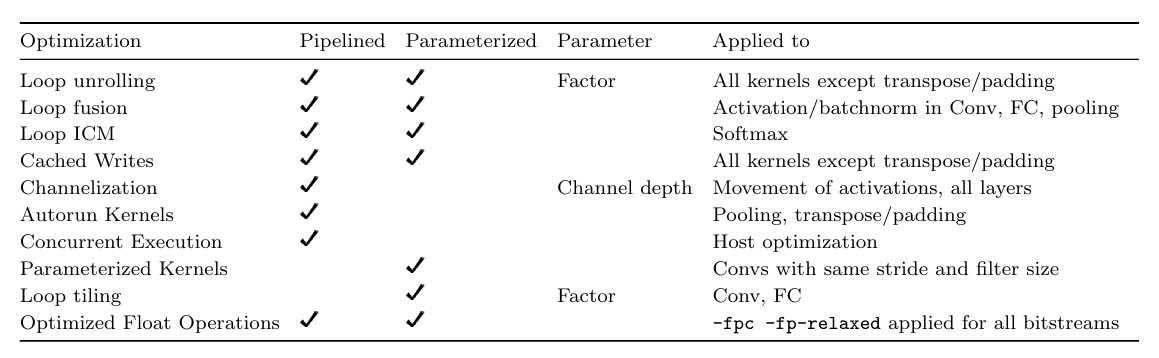
\includegraphics[width=\textwidth]{Images/CNNAccelerator/OptimizingCompiler-GeneratedOpenCLforCNNs/optimization_summary.png}
    \vspace{10pt} % Thay đổi giá trị 10pt theo nhu cầu
    \caption{Các phương pháp tối ưu hóa và khả năng áp dụng của chúng}
\end{figure}
\subsubsection{Triển khai}
\paragraph{Schedule Optimization}
\begin{itemize}
    \item Lớp Convolution: Schedule được tối ưu hóa bao gồm unrolling vòng lặp giảm, tiling dọc theo kênh FM đầu vào và cột FM đầu ra và unrolling các vòng lặp bên trong.
    \item Lớp fully-connected (FC): Lịch biểu được tối ưu hóa liên quan đến việc khai thác vòng lặp bên trong để tối đa hóa việc sử dụng bộ nhớ toàn cục và unrolling vòng lặp bên trong.
    \item Lớp Softmax: Lịch biểu được tối ưu hóa bao gồm việc kết hợp các vòng lặp để tính toán giá trị tối đa và tổng hàm mũ.
\end{itemize}
\paragraph{Custom Host Code}
Một chương trình máy chủ OpenCL C/C++ được triển khai bên ngoài TVM để hỗ trợ các tối ưu hóa không được hỗ trợ trong mã tạo máy chủ TVM.
\paragraph{Symbolic Shape Execution}
Tính năng này được sử dụng để nhóm việc thực thi các phép chập có cùng bước và kích thước bộ lọc vào cùng một kernel, cho phép sử dụng lại kernel và giảm mức sử dụng tài nguyên.
\subsubsection{Đánh giá}
\paragraph{Phương pháp}
\begin{itemize}
    \item Ba mạng CNN (LeNet-5, MobileNetV1 và ResNet-18/34) được triển khai trên ba nền tảng FPGA (Intel Arria 10, Stratix 10 MX và Stratix 10 SX).
    \item Hiệu suất được so sánh với các triển khai được tối ưu hóa cao trên CPU và GPU.
    \item Các chỉ số hiệu suất bao gồm FPS (Frames per second), GFLOPS (Floating-point operations per second) và mức sử dụng tài nguyên.
\end{itemize}
\paragraph{Nền tảng}
Thực hiện thí nghiệm với 3 nền tảng sau:
\begin{itemize}
    \item FPGA: Intel Arria 10 GX, Stratix 10 SX và Stratix 10 MX.
    \item CPU: Intel Xeon Platinum 8280.
    \item GPU: NVIDIA GTX 1060.
\end{itemize}
\paragraph{Hiệu suất suy luận}
\textbf{LeNet-5}:
Kết quả được hiển thị ở bên dưới:
\begin{figure}[!h]
    \centering
    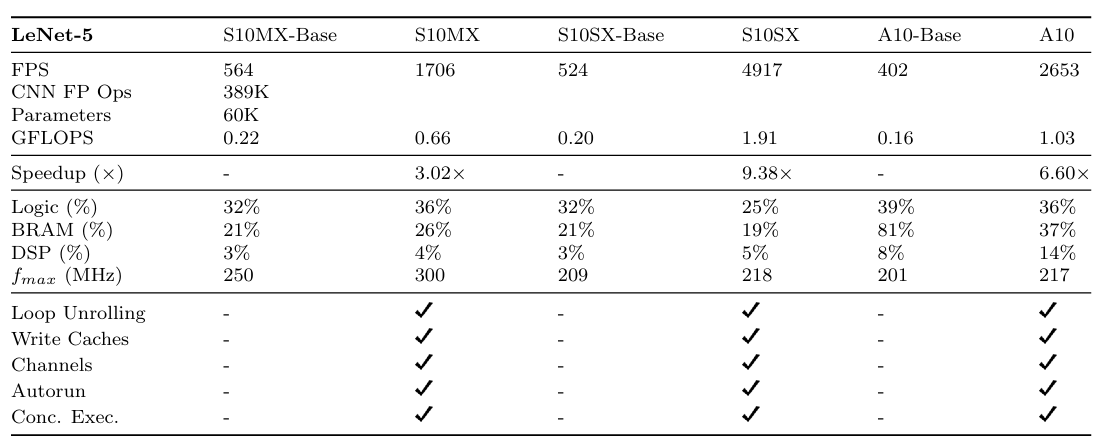
\includegraphics[width=\textwidth]{Images/CNNAccelerator/OptimizingCompiler-GeneratedOpenCLforCNNs/lenet5_inference.png}
    \vspace{10pt} % Thay đổi giá trị 10pt theo nhu cầu
    \caption{Kết quả khi hiện thực LeNet-5}
\end{figure}
\begin{itemize}
    \item FPGA đạt hiệu suất từ 1.59$\times$ đến 4.57$\times$ so với TF-CPU, 0.73$\times$ đến 2.10$\times$ so với TVM-1T và 1.06$\times$ đến 3.07$\times$ so với TF-cuDNN.
    \item Kết luận: Các bitstream FPGA được tối ưu hóa mang lại hiệu năng vượt trội so với CPU và cạnh tranh với GPU.
\end{itemize}
\textbf{MobileNetV1}
Kết quả được hiển thị ở bên dưới:
\begin{figure}[!h]
    \centering
    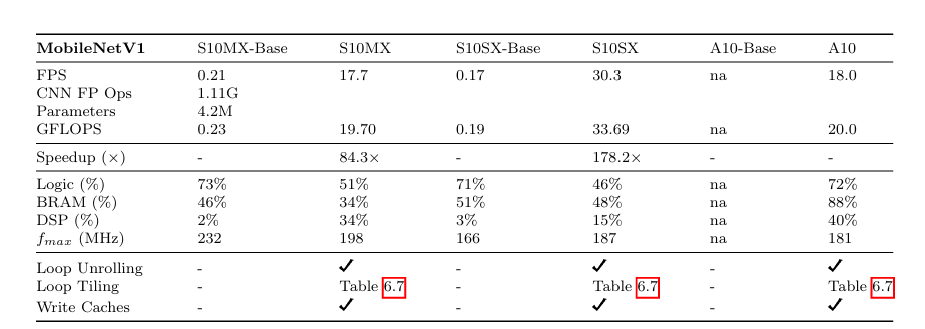
\includegraphics[width=\textwidth]{Images/CNNAccelerator/OptimizingCompiler-GeneratedOpenCLforCNNs/mobilenet.png}
    \vspace{10pt} % Thay đổi giá trị 10pt theo nhu cầu
    \caption{Kết quả khi hiện thực MobileNetV1}
\end{figure}
\begin{itemize}
    \item FPGA đạt hiệu suất từ 0.82$\times$ đến 1.40$\times$ so với TF-CPU, 1.13$\times$ đến 1.94$\times$ so với TVM-1T và chậm hơn từ 0.41$\times$ đến 0.69$\times$ so với TF-cuDNN.
    \item Kết luận: FPGA mang lại hiệu năng cạnh tranh với CPU và chậm hơn GPU, hiệu suất bị giới hạn bởi việc sử dụng DSP thấp và hiệu suất của các lớp khác.
\end{itemize}
\textbf{ResNet}
Kết quả được hiển thị ở bên dưới:
\begin{figure}[!h]
    \centering
    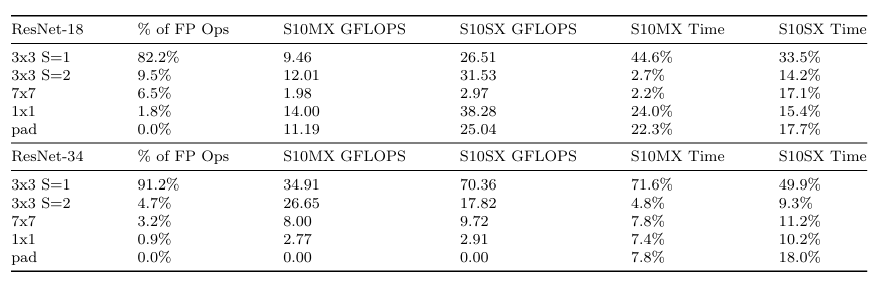
\includegraphics[width=\textwidth]{Images/CNNAccelerator/OptimizingCompiler-GeneratedOpenCLforCNNs/resnet.png}
    \vspace{10pt} % Thay đổi giá trị 10pt theo nhu cầu
    \caption{Kết quả khi hiện thực ResNet}
\end{figure}
\begin{itemize}
    \item FPGA chậm hơn CPU và GPU.
    \item Kết luận: Hiệu suất bị giới hạn bởi việc sử dụng DSP thấp và hiệu suất của các lớp khác.
\end{itemize}
\subsubsection{Hạn chế}
\begin{itemize}
    \item Sử dụng khối DSP thấp: Việc triển khai bị giới hạn bởi khả năng sử dụng DSP tối đa đạt được, đặc biệt là đối với các mạng lớn hơn.
    \item Suy giảm Fmax: Việc lát gạch và trải cuộn vòng lặp có thể dẫn đến suy giảm fmax do tăng độ phức tạp của việc định tuyến.
    \item Hiệu suất của các lớp khác: Hiệu suất của các phép cuộn 3x3 chiều sâu, đệm, softmax, và các lớp dày đặc hiện đang giới hạn hiệu suất tổng thể.
\end{itemize}
\section{Kiến trúc tăng tốc CNN gắn với RISC-V}
\subsection{RoCC, DMA và tổ chức GEMM}
Nghiên cứu của He là đối chiếu chính về đường tích hợp CPU--accelerator. Phần kiến trúc mô tả Rocket Core kết nối bộ tăng tốc qua RoCC; bộ tăng tốc dùng DMA để đọc/ghi feature map qua L2 cache và DRAM. Khối điều khiển, khối tính toán và khối lưu trữ cục bộ cho phép phân biệt việc phát lệnh của CPU với di chuyển dữ liệu của phần cứng~\cite[Section~3, Figure~4]{he2021design}. Khác với cơ chế này, trong MyTinyMobileNetSoC, CPU phải đọc tensor rồi ghi toán hạng qua MMIO; ngoại vi không có đường DMA tới RAM.

Khối tính toán của He kết hợp GEMM với mảng systolic giữ trọng số tại các phần tử xử lý (weight-stationary). Các PE hợp thành tile; thanh ghi giữa các tile tổ chức đường ống. Trọng số được nạp trước rồi dùng với luồng đầu vào, trong khi chia khối phép nhân ma trận nhằm giảm truy cập lặp~\cite[Sections~2.2--3, Figure~5]{he2021design}. Phạm vi mô tả tập trung vào tăng tốc tích chập bằng tính toán ma trận; sơ đồ có khối activation/pooling, nhưng bài không mô tả đủ để xác nhận một đường depthwise chuyên biệt hoặc toàn bộ hậu xử lý giống firmware của luận văn.

Đặt cạnh thiết kế này, Conv/Depthwise/Pointwise của MyTinyMobileNetSoC biểu diễn các phép tính theo cấu trúc toán tử thay vì một mảng GEMM chung. Firmware quyết định khi nào giữ patch, nạp trọng số và sử dụng kết quả cho từng shape. Phương án ma trận có thể dùng chung lõi tính toán cho nhiều lớp, đổi lại yêu cầu ánh xạ tensor và cấp dữ liệu đủ đều. Phương án chuyên biệt giảm nhu cầu ánh xạ qua ma trận trong đường chạy hiện tại, nhưng có phạm vi shape và các nhánh fallback phải kiểm chứng. Hai cách tổ chức đặt sự phức tạp ở những vị trí khác nhau.

\subsection{Giới hạn bằng chứng và ý nghĩa đối chiếu}
Phần thực nghiệm của He sử dụng YOLOv3-tiny và báo cáo thời gian xử lý trên nền tảng FPGA~\cite[Section~4]{he2021design}. Tuy nhiên, sơ đồ kiến trúc ghi Rocket Core còn phần kết luận nêu BOOM hai lõi. Vì thế, chương chỉ dùng Rocket/RoCC để chỉ phương án kết nối được mô tả, không coi đây là cấu hình host đã được xác nhận nhất quán cho toàn bộ số đo. Bài cũng không công bố rõ độ rộng toán hạng và tích lũy của cấu hình đánh giá, nên không gán INT8/INT32 cho thiết kế này.

Sự khác nhau về workload, host và hệ thống nhớ không cho phép xếp hạng từ FPS được báo cáo. Giá trị đối chiếu nằm ở mức tự chủ: với DMA, CPU có thể giao tác vụ có kích thước lớn hơn cho accelerator; với MMIO do CPU cấp dữ liệu, chi phí mỗi lần gọi và lượng dữ liệu hữu ích mỗi giao dịch trở thành mục tiêu tối ưu trực tiếp. Đây là cơ sở để Chương~\ref{chap:kientruc} làm rõ ranh giới giao diện và Chương~\ref{chap:toiuu} đánh giá cả phần truyền dữ liệu của MyTinyMobileNetSoC.

\section{Hướng tăng tốc tổng quát bằng mảng systolic/GEMM}
ConvAU của Kiningham, Graczyk và Ramkumar đại diện cho hướng lấy nhân ma trận đặc làm trung tâm. Thiết kế dùng phép nhân 8 bit và tích lũy 32 bit, giữ trọng số tại PE, cấp đầu vào qua FIFO SRAM và lưu kết quả trung gian trong hệ thống đệm. Host nạp trọng số cùng metadata lượng tử hóa; phần cứng đảm nhiệm tính toán ma trận, lượng tử hóa và ReLU. Báo cáo không xác định một lõi RISC-V hoặc giao thức MMIO/RoCC tương ứng, nên không thể xem ConvAU là một SoC cùng cấu hình với luận văn~\cite[Sections~3--4]{kiningham2016design}.

\subsection{Thông lượng, chuẩn bị dữ liệu và mức sử dụng mảng}
Dòng MAC đều đặn cho phép tái sử dụng toán hạng qua các PE và khai thác song song khi kích thước ma trận phù hợp. Tuy nhiên, tích chập cần được ánh xạ sang phép nhân ma trận. ConvAU trình bày phép biến đổi im2col để sắp cửa sổ đầu vào thành cột~\cite[Section~4.2]{kiningham2016design}. Nếu vật chất hóa ma trận đó, các phần tử cửa sổ chồng lấn bị lặp, làm tăng lưu trữ và lưu lượng; nếu sinh dữ liệu theo luồng, chi phí chuyển sang bộ tạo địa chỉ và bộ đệm. Vì vậy, so sánh phải tính cả chuẩn bị dữ liệu, nạp trọng số, làm đầy và tháo cạn đường ống.

Đối với workload của luận văn, pointwise có cấu trúc trộn kênh phù hợp phép nhân ma trận, còn depthwise tính độc lập từng kênh~\cite[Section~3.1]{howard2017mobilenets}. Từ cấu trúc đó có thể suy ra rằng ánh xạ depthwise hoặc ma trận nhỏ lên mảng đặc lớn cần lịch ghép tác vụ hay chia khối phù hợp để tránh nhiều PE không có việc hữu ích. Đây là nhận xét về điều kiện sử dụng mảng, không phải số đo mức sử dụng của ConvAU trên TinyMobileNet và cũng không có nghĩa mọi mảng systolic đều xử lý depthwise kém.

\subsection{Phạm vi đánh giá và bài học cho hệ thống hiện tại}
ConvAU được đánh giá bằng RTL, tổng hợp và luồng ASIC, với SqueezeNet lượng tử hóa làm workload~\cite[Section~5]{kiningham2016design}. Thông lượng và công suất trong báo cáo thuộc điều kiện đó; không dùng chúng để suy ra ưu thế năng lượng hoặc độ trễ của FPGA trong luận văn. So sánh số bit cũng chỉ là một tiêu chí: cùng độ rộng tensor và tích lũy chưa bảo đảm quy tắc làm tròn hay saturation giống nhau.

Khác với ConvAU, MyTinyMobileNetSoC không thực hiện mạng bằng một mảng ma trận đặc chung và không dựng ma trận im2col đầy đủ trong đường chạy hiện tại. Dữ liệu được chuẩn bị theo patch hoặc vector kênh cho ngoại vi chuyên biệt. Lựa chọn này phù hợp phạm vi hiện thực TinyMobileNet đã xác định, nhưng đánh đổi bằng lịch firmware phụ thuộc shape và phần tính toán còn ở CPU. Bài học từ hướng systolic là phải cân đối số MAC với khả năng nuôi dữ liệu và miền tái sử dụng, thay vì xem kích thước mảng là thước đo đủ cho hiệu năng hệ thống.

\section{Tổng hợp so sánh và vị trí của MyTinyMobileNetSoC}
\label{sec:related-position}
Bảng~\ref{tab:related-integration} và Bảng~\ref{tab:related-scope} dùng cùng tập công trình để đối chiếu hai nhóm tiêu chí: tích hợp/luồng dữ liệu và phạm vi/số học. Các nhận xét ở cột cuối là tổng hợp kiến trúc của chương; chúng không biểu thị thứ hạng. Khi nguồn không xác định rõ một thuộc tính, bảng ghi giới hạn đó thay vì suy đoán từ tên nền tảng.

\begingroup
\small
\setlength{\tabcolsep}{4pt}
\renewcommand{\arraystretch}{1.12}
\begin{longtable}{@{}>{\raggedright\arraybackslash}p{0.17\textwidth}>{\raggedright\arraybackslash}p{0.23\textwidth}>{\raggedright\arraybackslash}p{0.28\textwidth}>{\raggedright\arraybackslash}p{0.26\textwidth}@{}}
\caption{So sánh host, kiểu tăng tốc và truyền dữ liệu}\label{tab:related-integration}\\
\toprule
Công trình & CPU/host và kiểu tăng tốc & Điều khiển, truyền dữ liệu & Miền tái sử dụng chính \\
\midrule
\endfirsthead
\toprule
Công trình & CPU/host và kiểu tăng tốc & Điều khiển, truyền dữ liệu & Miền tái sử dụng chính \\
\midrule
\endhead
\bottomrule
\endfoot
Ge và cộng sự~\cite{ge2019compact} & Cortex-M3; chuỗi tích chập, kích hoạt, pooling & AHB tới accelerator; điều khiển và bank nhớ nội bộ & Buffer cửa sổ; chia sẻ nguồn giữa chuỗi; bank luân phiên giữ tổng riêng/kết quả \\
\midrule
He~\cite{he2021design} & Sơ đồ Rocket; GEMM/systolic giữ trọng số & RoCC điều khiển; DMA tới L2/DRAM & Trọng số tại PE; tile ma trận và lưu trữ cục bộ \\
\midrule
ConvAU~\cite{kiningham2016design} & Host không xác định lõi; mảng nhân ma trận đặc & Host nạp trọng số/metadata; không xác định giao thức bus SoC & Trọng số tại PE; FIFO đầu vào và đệm trung gian \\
\midrule
Chung~\cite{chung2021optimization} & Host OpenCL; kernel FPGA sinh từ TVM & Runtime, buffer toàn cục, hàng đợi; kênh giữa kernel khi pipeline & Tiling, lưu cục bộ, fusion và tái dùng kernel khi folded \\
\midrule
MyTiny\-Mobile\-NetSoC (Chương~\ref{chap:kientruc}) & PicoRV32; ngoại vi Conv, Depthwise, Pointwise, Quant & MMIO qua bus gốc; CPU chuyển toán hạng; không DMA; RAM mã/dữ liệu 256~KiB & Patch/tile và cache trọng số chuyên biệt, do firmware lập lịch theo shape \\
\end{longtable}
\endgroup

\begingroup
\small
\setlength{\tabcolsep}{4pt}
\renewcommand{\arraystretch}{1.12}
\begin{longtable}{@{}>{\raggedright\arraybackslash}p{0.17\textwidth}>{\raggedright\arraybackslash}p{0.18\textwidth}>{\raggedright\arraybackslash}p{0.26\textwidth}>{\raggedright\arraybackslash}p{0.33\textwidth}@{}}
\caption{So sánh số học, phạm vi đánh giá và khác biệt với luận văn}\label{tab:related-scope}\\
\toprule
Công trình & Số học & Phạm vi và bằng chứng & Khác biệt chính so với luận văn \\
\midrule
\endfirsthead
\toprule
Công trình & Số học & Phạm vi và bằng chứng & Khác biệt chính so với luận văn \\
\midrule
\endhead
\bottomrule
\endfoot
Ge và cộng sự~\cite{ge2019compact} & Fixed-point 10 bit; tổng riêng 32 bit & SoC FPGA; đánh giá LeNet-5 & Nhiều bước xử lý và buffering nằm trong accelerator; không xác nhận đường depthwise riêng \\
\midrule
He~\cite{he2021design} & Không nêu rõ độ rộng cấu hình đánh giá & FPGA; YOLOv3-tiny; phần kết luận nêu BOOM khác host trong sơ đồ & Tập trung nhân ma trận và DMA; không đủ chi tiết để đồng nhất cấu hình số học/host của số đo \\
\midrule
ConvAU~\cite{kiningham2016design} & Nhân 8 bit; tích lũy 32 bit & RTL và luồng ASIC; SqueezeNet lượng tử hóa & Ánh xạ CNN sang ma trận; phần cứng có ReLU/lượng tử hóa; không phải đánh giá SoC FPGA cùng điều kiện \\
\midrule
Chung~\cite{chung2021optimization} & Dấu phẩy động & OpenCL FPGA; LeNet-5, MobileNetV1, ResNet & Tối ưu trình biên dịch và runtime; không cấp toán hạng từng phép qua MMIO \\
\midrule
MyTiny\-Mobile\-NetSoC (Chương~\ref{chap:kientruc}, \ref{chap:toiuu}) & Tensor INT8; tích lũy INT32 & TinyMobileNet/MNIST; mô phỏng và đánh giá FPGA post-route cho ZCU106 & Tích hợp và lịch firmware theo workload; còn fallback CPU; chưa xác nhận suy luận trên bo mạch \\
\end{longtable}
\endgroup

\subsection{Ranh giới tích hợp và phạm vi tối ưu được chọn}
Từ các đối chiếu trên, lựa chọn của luận văn là một hệ thống mà trách nhiệm truyền dữ liệu còn tường minh ở CPU. PicoRV32 đọc tensor từ RAM dùng chung, nạp các thanh ghi ngoại vi và thu kết quả. RAM 256~KiB là bộ nhớ chung cho mã và dữ liệu của CPU; các bộ tăng tốc không có cổng tự truy cập RAM. Conv, Depthwise, Pointwise và Quant là các đường được firmware sử dụng; SoC còn có bộ nhân độc lập nhưng đường suy luận hiện tại không sử dụng nó (Chương~\ref{chap:kientruc}).

Phạm vi tăng tốc không bao phủ mọi phép toán của mạng. Trong thiết kế cuối, Conv0, DW1, DW2 và các lớp Pointwise có đường tích lũy phần cứng; DW3, GAP và FC vẫn dùng số học CPU. Requantization dùng ngoại vi Quant, còn CPU chịu trách nhiệm bias, offset đầu ra, clamp và điều phối lớp. Trọng số và feature map là INT8, bias và tích lũy là INT32; điều đó không tự xác nhận tương đương từng bit với các hệ lượng tử hóa khác. Phân công cụ thể được làm rõ trong Chương~\ref{chap:kientruc}, tránh đồng nhất tên ngoại vi với mức bao phủ toàn bộ toán tử.

So với bộ đồng xử lý DMA hoặc mảng GEMM chung, phạm vi tối ưu ở đây tập trung vào giao dịch MMIO, lịch vòng lặp và lưu giữ dữ liệu theo shape của TinyMobileNet. Đổi lại, việc chuyên biệt hóa cần điều kiện chọn nhánh, fallback và kiểm tra giao dịch tương ứng. Kết quả được đánh giá bằng điểm số/dự đoán, số chu kỳ và tài nguyên/timing post-route trên mục tiêu ZCU106 ở Chương~\ref{chap:toiuu}. Flow hiện có chưa xác nhận suy luận TinyMobileNet trên bo mạch và chưa có số đo năng lượng để đối chiếu các công trình trước.

Các nghiên cứu được giữ lại làm rõ những lựa chọn đã có về phân công, lưu trữ và lập lịch; chúng không đủ cơ sở để khẳng định tính mới hoặc ưu thế phổ quát của MyTinyMobileNetSoC. Vị trí của đề tài là hiện thực và đánh giá một phương án tích hợp cụ thể, trong đó hiệu năng phụ thuộc đồng thời vào datapath chuyên biệt và cách CPU phục vụ dữ liệu. Từ những lựa chọn này, Chương~\ref{chap:kientruc} trình bày kiến trúc được chọn, giao diện MMIO và đường suy luận thực tế của hệ thống.

